\documentclass{article}
\usepackage{style}
\title{COURSECODE Cheatsheet}
\author{Hanhee Lee}
\lhead{COURSECODE}
\rhead{Hanhee Lee}

\begin{document}
    \maketitle

    \tableofcontents

    \listoffigures

    \listoftables

    \section{Week 1}
    \begin{terminology}
        \textbf{Interest Rate}
        \begin{enumerate}
            \item \(P\): Principle amount
            \item \(F\): Future amount 
            \item \(F_N\) : Future amount in (time unit) \(N\)
            \item \(N\): Number of periods (e.g. years)
            \item \(i\): Interest rate 
            \item \(I\): Total interest amount 
            \item \(r\) Nominal interest rate (usually for 1 year)
            \item \(m\): Number of times compounded (subperiods) per year
            \item \(i_s\): Subperiod interest rate
            \item \(i_e\): Effective interest rate, the equivalent rate if compounded only once per year.
        \end{enumerate}
    \end{terminology}

    \begin{definition}
        \textbf{Interest Rate}
        \begin{equation}
            i = \frac{I}{P}
        \end{equation}
    \end{definition}

    \begin{definition}
        \textbf{Subperiod Interest Rate}
        \begin{equation}
            i_s = \frac{r}{m}
        \end{equation}
    \end{definition}

    \begin{definition}
        \textbf{Effective Interest Rate}
        \begin{equation}
            i_e = (1 + i_s)^m - 1
        \end{equation}
    \end{definition}
    
    \begin{definition}
        \textbf{Simple Interest} 
        \begin{equation}
            F_N = P(1 + Ni)
        \end{equation}
    \end{definition}

    \begin{definition}
        \textbf{Compound Interest} 
        \begin{equation}
            F_N = P(1 + i)^N
        \end{equation}
    \end{definition}

    \begin{definition}
        \textbf{Compound Interest with Subperiods} 
        \begin{equation}
            F_N = P(1 + i_s)^{Nm}
        \end{equation}
    \end{definition}

    \begin{definition}
        \textbf{Continuous Compound Interest} The finite amount of \(i_e\) as the compounding period becomes infinitesimally small.
        \begin{equation}
            i_e = \lim_{m \to \infty} (1 + \frac{r}{m})^m - 1 = e^r - 1
        \end{equation}
        \textbf{Note:} \(i_e\) increases as the compounding period decreases.
    \end{definition}

    \section{Week 2}


    \section{Week 3}

    \section{Week 4}

    \section{Week 5}

    \section{Week 6}

    \section{Week 7}

    \section{Week 8}

    \section{Week 9}

    \section{Week 10}

    \section{Week 11}

    \section{Week 12}

    \section{Week 13}

% Process
\begin{process}
    \begin{enumerate}
        \item 
        \item 
        \item 
        \item 
    \end{enumerate}
\end{process}

% Example 
\begin{example}
    Hanhee Lee
\end{example}

% Definition
\begin{definition}
    
\end{definition}

% Theorem
\begin{theorem}
    Hanhee Lee
\end{theorem}

% Derivation
\begin{derivation}
    Hanhee Lee
\end{derivation}

% Intuition
\begin{intuition}
    Hanhee Lee
\end{intuition}

% Warning
\begin{warning}
    Hanhee Lee
\end{warning}

% Summary
\begin{summary}
    Hanhee Lee
\end{summary}

% Insert Image 
\begin{figure}[H]
    \centering
    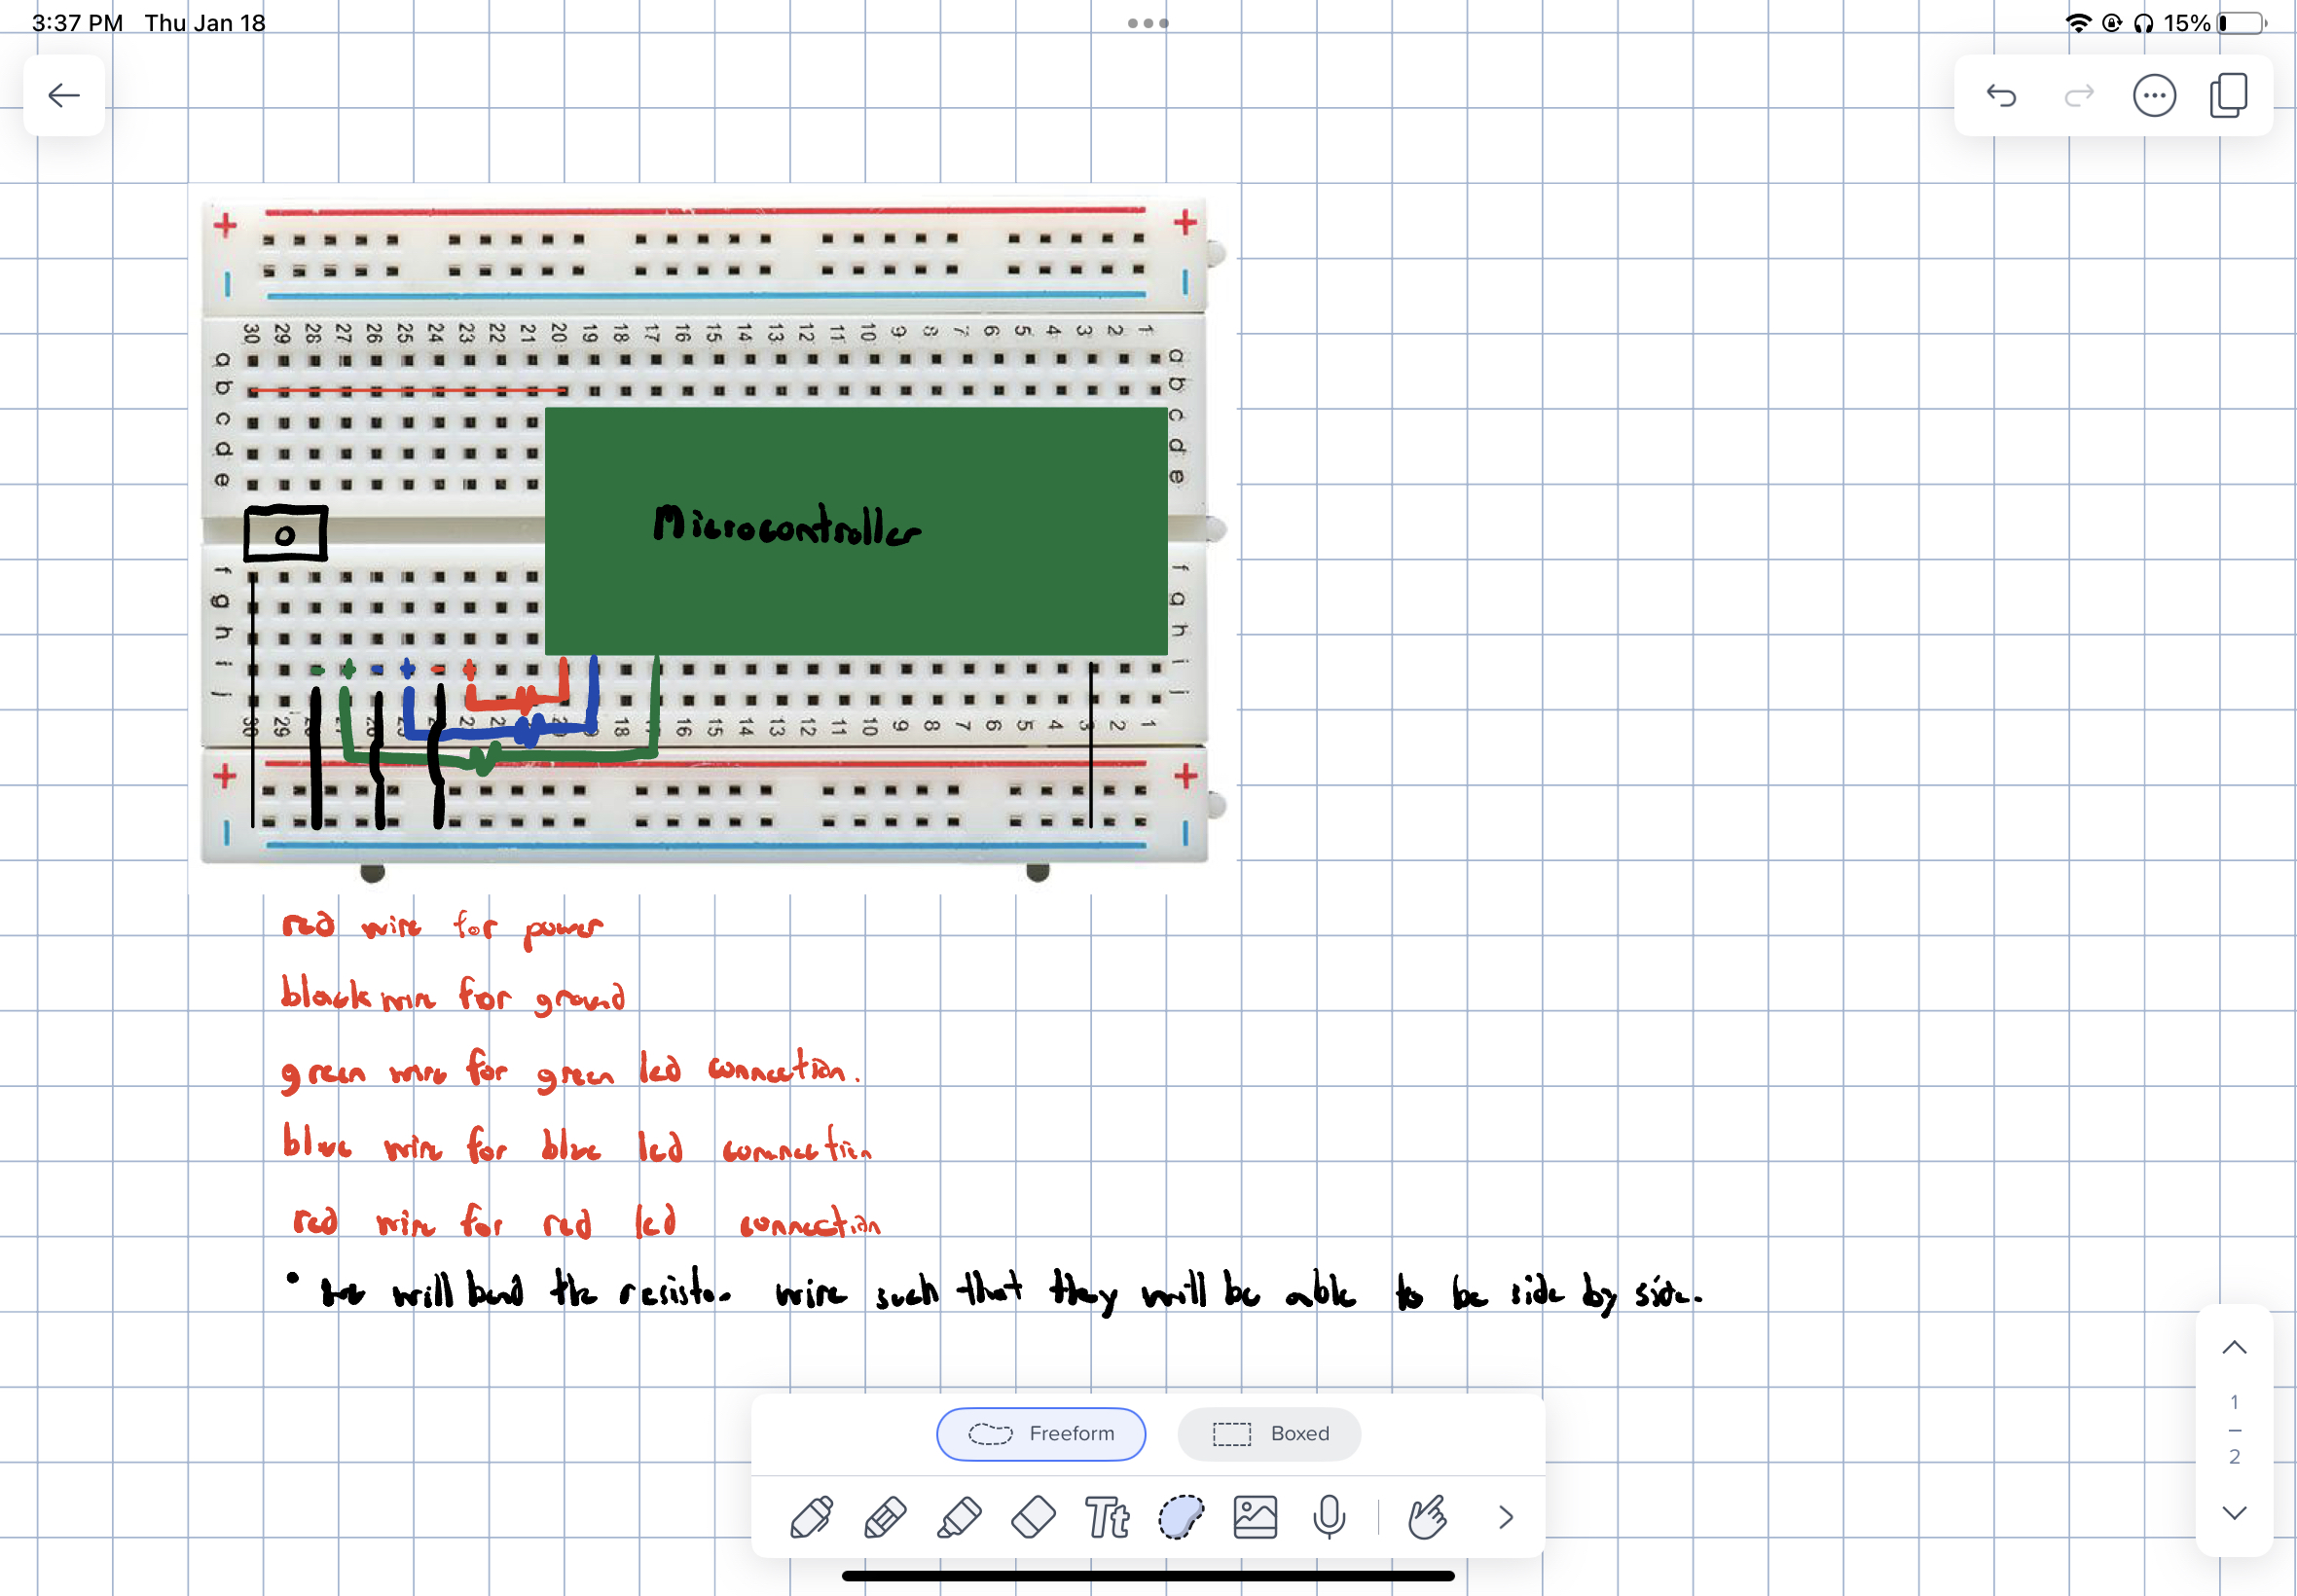
\includegraphics[width=0.5\textwidth]{00_Images/diagram_circuit.png}
    \caption{ESC195}
\end{figure}

\end{document}